\begin{appendices}
% \crefalias{chapter}{appsec}
% \chapter{Heat Equation Derivation}
% \label{app:heatderive}

% To derive the heat equation we consider the conversation of energy in a volume R, with a flux out, $\phi(x,y,z,t)$, and unit outer normal $\mathbf{\hat{n}}$. We need just the normal component of $\phi$ 
% : $\phi \cdot \mathbf{\hat{n}}$.
% \medskip

% The rate of change of heat inside the volume R is equal to the heat generated inside the volume R plus the heat flowing in/out of the boundary surface:

% \begin{equation}
% \parbox{70pt}{Rate of change of heat energy}\ =\ \parbox{60pt}{Rate of heat generation in R} +\ \parbox{105pt}{Rate of heat energy flowing through boundary surface}
% \label{eqn:word}
% \end{equation}

% \medskip
% The total heat energy is:

% \begin{equation}
% e(x,y,z,t)=c(x,y,z)\cdot \rho(x,y,z)\cdot T(x,y,z,t)
% \end{equation} 

% and therefore the rate of change of heat energy is

% \begin{equation}
% \frac{d}{dt} \iiint\limits_{R} e\ dV= \frac{d}{dt}\iiint\limits_{R} c\rho T\ dV
% \label{eqn:rotenergy}
% \end{equation}

% We denote the heat generated inside the volume R as $Q(x,y,z,t)$:

% \begin{equation}
% \iiint\limits_{R} Q\ dV
% \label{eqn:rotheatgen}
% \end{equation}

% and the rate of heat energy flowing through the boundary surface is:

% \begin{equation}
% -\iint \limits_{\partial R} \phi\cdot \mathbf{\hat{n}}\ dS\footnote[3]{This is negative as outward flow $\phi$ is positive, but the flow would result in a reduction of energy.}
% \label{eqn:rotheatloss}
% \end{equation}

% Substituting \cref{eqn:rotenergy,eqn:rotheatgen,eqn:rotheatloss} into \cref{eqn:word}, yields:

% \begin{equation}
% \frac{\partial}{\partial t} \iiint\limits_{R} c\rho T\ dV = -\iiint \limits_{R} \phi\cdot \mathbf{\hat{n}}\ dV +  \iiint\limits_{R} Q\ dV
% \end{equation}

% Using the divergence theorem, and simplifying gives: 

% %\begin{equation}
% %\iint \limits_{\partial R} \phi\cdot \mathbf{\hat{n}}\ dS = \iiint \limits_{R} \nabla\cdot \phi\ dV
% %\end{equation}

% \begin{equation}
% \frac{\partial}{\partial t} \iiint\limits_{R} c\rho T\ dV = -\iiint \limits_{R} \nabla\cdot \phi\ dV +  \iiint\limits_{R} Q\ dV
% \end{equation}

% \begin{equation}
% \iiint\limits_{R} \left[ c\rho \frac{\partial}{\partial t} T + \nabla\cdot \phi - Q\right] dV = 0
% \end{equation}

% Which holds for an arbitrary R, thus:

% \begin{equation}
% c\rho\frac{\partial}{\partial t}T = - \nabla \cdot \phi + Q
% \label{eqn:heatpreq}
% \end{equation}



% Using Fourier's law of heat conduction, which states that the local heat flux density, $\phi$, is proportional to the negative local temperature gradient. The proportionality constant being equal to the thermal conductivity, $\kappa$:

% \begin{equation}
% \phi(x,y,z,t)=\kappa(x,y,z)\nabla T(x,y,z,t)
% \label{eqn:fourier}
% \end{equation}

% Substituting \cref{eqn:fourier} into \cref{eqn:heatpreq} yields the heat equation:

% \begin{equation}
% c\rho\frac{\partial}{\partial t}T = \nabla\cdot (\kappa\nabla T) + Q
% \end{equation}

% Which can be simplified into the homogeneous medium heat equation with the following assumptions: Q=0 and $\kappa,\ \rho,\ and\ c$ are constant, and $\alpha=\tfrac{\kappa}{c\rho}$

% \begin{equation}
% \frac{\partial T}{\partial t} = \alpha \nabla^2 T
% \end{equation}


\crefalias{chapter}{appsec}
\chapter{Detected Light Fluence Tracking Method}
\label{app:lightdect}

Most the fluence graphs presented in this thesis shows the fluence of the incident light throughout the simulated medium.
However, there are problems where tracking the fluence of the detected light maybe useful, though this quantity is not straight forward to track.
The current method of tracking fluence, is to add pathlengths, calculated as the packet moves from voxel to voxel to a 3D array. 
This method obviously cannot determine which packet will be detected before the packet is detected, therefore a new method must be devised.
This new method tracks the coordinates, direction vectors, random optical distance and fluorescent source of the packet using a stack.
A stack is a commonly used abstract data structure, and is a collection of elements.
In this case the elements are the coordinates, direction vectors, optical distance and fluorescent source.
A stack has two main operations, pop and push.
The push operation adds a new element to the collection, and the pop operation removes the most recently added element from the collection.
This is known as last in first out (LIFO).
\Cref{fig:stack} shows these two operations in action.

\begin{figure}[!htpb]
	\centering
	\includegraphics[width=0.35\textwidth]{stack.pdf}
	\caption{Example of the push and pop operation on a stack. The first operation add the integer 2 to the stack. The second operation push 7 to the stack. The last operation pops the 7 from the stack.}
	\label{fig:stack}
\end{figure}

The progress of each packets is pushed onto the stack, as it is propagated through the simulated medium. 
As mentioned above the packets coordinates, direction vectors, optical depth, and fluorescent source are the quantities pushed to the stack.
These quantities are pushed to stack every time an interaction event occurs.
When a packet is terminated, either via absorption or it leaving the medium, the packets details are removed from the stack.
This occurs unless the packet is detected.
If the packet is detected then the information remains on the stack.
This whole process repeats until all the packets have been run.
Once all the packets have been run, the packets are ``replayed''.
This is achieved by popping the information off the stack and passed to the inttau2 routine.
The packet is the propagated again, this time recording the fluence as done in most of the chapters in this thesis.

\end{appendices}
